\chapter{Comparison and Discussion}
\label{ch:comparison}

\section{Holdout evaluation protocol}
\label{sec:comparison-protocol}

All three methods of Chapters~\ref{ch:kriging}, \ref{ch:gbm}
and~\ref{ch:bayesnf} (Ordinary Kriging, gradient boosting and Bayesian
Neural Fields) are evaluated on the same fully held-out subset of the
ReKIS network. Before any model fitting, the 2{,}458 quality-controlled
stations are split into 1{,}966 training stations and 492 holdout
stations. The split is identical across the three methods; the holdout
assignment is stored in \texttt{kriging/holdout\_station\_ids.json} on the
project bucket and is consumed by all three evaluation notebooks.

Models are trained on the 1{,}966 training stations only. The holdout
stations are used only at evaluation time, on which CRPS and MAE are
reported in physical millimetres. The predicted-wet rows below restrict
the evaluation to records on which the model predicts rainfall above
$0{.}4$~mm (${\approx}41\,\%$ of the records).

The three methods do not share a common evaluation window. Ordinary
Kriging and gradient boosting are evaluated on the full $1961$--$2023$
record. Bayesian Neural Fields is evaluated on the $2014$--$2023$
ten-year window because training BayesNF at the canonical
hyperparameters of Section~\ref{sec:bayesnf-arch} (32~VI replicas
$\times$ 100 epochs on the long-table input) over the full $63$-year
record exceeded the GPU budget allocated to this thesis. The
$2014$--$2023$ subset is the same window used for the VI-vs-MAP
cross-validation of Section~\ref{sec:bayesnf-vi-vs-map} and corresponds
to the densest decade of the ReKIS network. The cross-method numbers
of Table~\ref{tab:final-comparison} must therefore be read with this
asymmetry in mind: the BayesNF row covers the recent dense decade
rather than the long historical tail of the record.

\section{Cross-model metrics}
\label{sec:comparison-metrics}

Table~\ref{tab:final-comparison} collects the final holdout metrics for
the three methods.

\begin{table}[ht]
  \centering
  \caption{Final holdout metrics on the 492 reserved stations.
  Predicted-wet rows include only records with $\hat{Z} \ge 0{.}4$~mm.
  Ordinary Kriging and gradient boosting are evaluated over the full
  $1961$--$2023$ record; Bayesian Neural Fields over the $2014$--$2023$
  decade only (Section~\ref{sec:comparison-protocol}).}
  \label{tab:final-comparison}
  \begin{tabular}{l l cc}
    \toprule
    Method & Subset & MAE (mm) & CRPS (mm) \\
    \midrule
    Ordinary Kriging   & All records   & 0.480 & 0.384 \\
    Ordinary Kriging   & Predicted-wet & 1.092 & 0.858 \\
    \midrule
    Gradient boosting  & All records   & 0.432 & 0.342 \\
    Gradient boosting  & Predicted-wet & 0.965 & 0.735 \\
    \midrule
    Bayesian Neural Fields & All records   & 0.347 & 0.286 \\
    Bayesian Neural Fields & Predicted-wet & 0.802 & 0.702 \\
    \bottomrule
  \end{tabular}
\end{table}

The ranking is consistent across both error families and across the
all-records and predicted-wet partitions of the holdout set. Bayesian
Neural Fields attains the lowest CRPS and the lowest MAE in every row
of Table~\ref{tab:final-comparison}: relative to Ordinary Kriging it
reduces all-records MAE by $27.7\,\%$ and CRPS by $25.5\,\%$, and
relative to gradient boosting it reduces the same metrics by $19.7\,\%$
and $16.4\,\%$. The improvement persists on the harder predicted-wet
subset, on which BayesNF cuts the kriging CRPS by $18.2\,\%$ and the
gradient-boosting CRPS by $4.5\,\%$. Even after the evaluation-window
caveat of Section~\ref{sec:comparison-protocol} is taken into account
(the BayesNF row is computed on the recent dense decade rather than on
the full historical record), the gap is large enough that the model
remains the strongest of the three on the common $2014$--$2023$ slice,
and it is the only method that produces a calibrated predictive
distribution at every grid cell rather than a point estimate plus a
plug-in variance. On these grounds the Bayesian Neural Field is
selected as the production model for the gridded precipitation product
of the next section.

\section{Multi-resolution gridded product}
\label{sec:comparison-multires}

The selected BayesNF model is applied over the full study domain to
produce a gridded daily precipitation product on the EPSG:3035
projection. Construction proceeds in three steps. First, the same
feature vector that the model expects at training time is recomputed
at every cell of a $1$~km EPSG:3035 lattice over the study area: the
static covariates (projected coordinates, latitude and longitude,
elevation from Copernicus DEM, the six SoilGrids variables) are
sampled once from the rasters, and the dynamic neighbour-derived
features (IDW, GOS and the five SVD-quantile levels
$\mathrm{svd}\_05..\mathrm{svd}\_09$ of
Section~\ref{sec:bayesnf-features}) are recomputed per day, using the
$1{,}966$ training stations as the neighbour pool so that no holdout
station enters the input. Second, the $1$~km feature parquets are
block-mean-aggregated to $2$, $5$ and $10$~km, so that all four nested
target grids share the same domain extent, origin and feature schema.
Third, the trained BayesNF VI ensemble of Chapter~\ref{ch:bayesnf},
fit on the $1{,}966$ training stations only, is run forward on every
(cell, day) feature row and emits a posterior predictive mean in
millimetres together with the standard deviation aggregated over the
$32$ VI replicas. The product is materialised for the month of
March~$2023$ as a worked example covering all four resolutions; the
same pipeline runs unchanged on any other date range.

Figure~\ref{fig:multires-case-day} compares the four resolutions on
the case day $2023$-$03$-$26$. As the cell size grows, two effects
are visible. The first is a progressive smoothing of orographic
gradients along the southern foothills: the sharp wet--dry contrast
that the $1$~km field resolves at the ridgeline is blurred at $5$~km
and largely flattened at $10$~km, because block-mean aggregation of
the input features averages the underlying elevation and neighbour
statistics over progressively larger windows. The second is the
gradual disappearance of small, isolated rain cells in the northern
plain: $1$--$2$~mm pockets that are individually resolved at $1$~km
get diluted into the surrounding dry background as soon as the cell
encompasses several of them, and by $10$~km they are no longer
distinguishable from the climatological field.

\begin{figure}[ht]
  \centering
  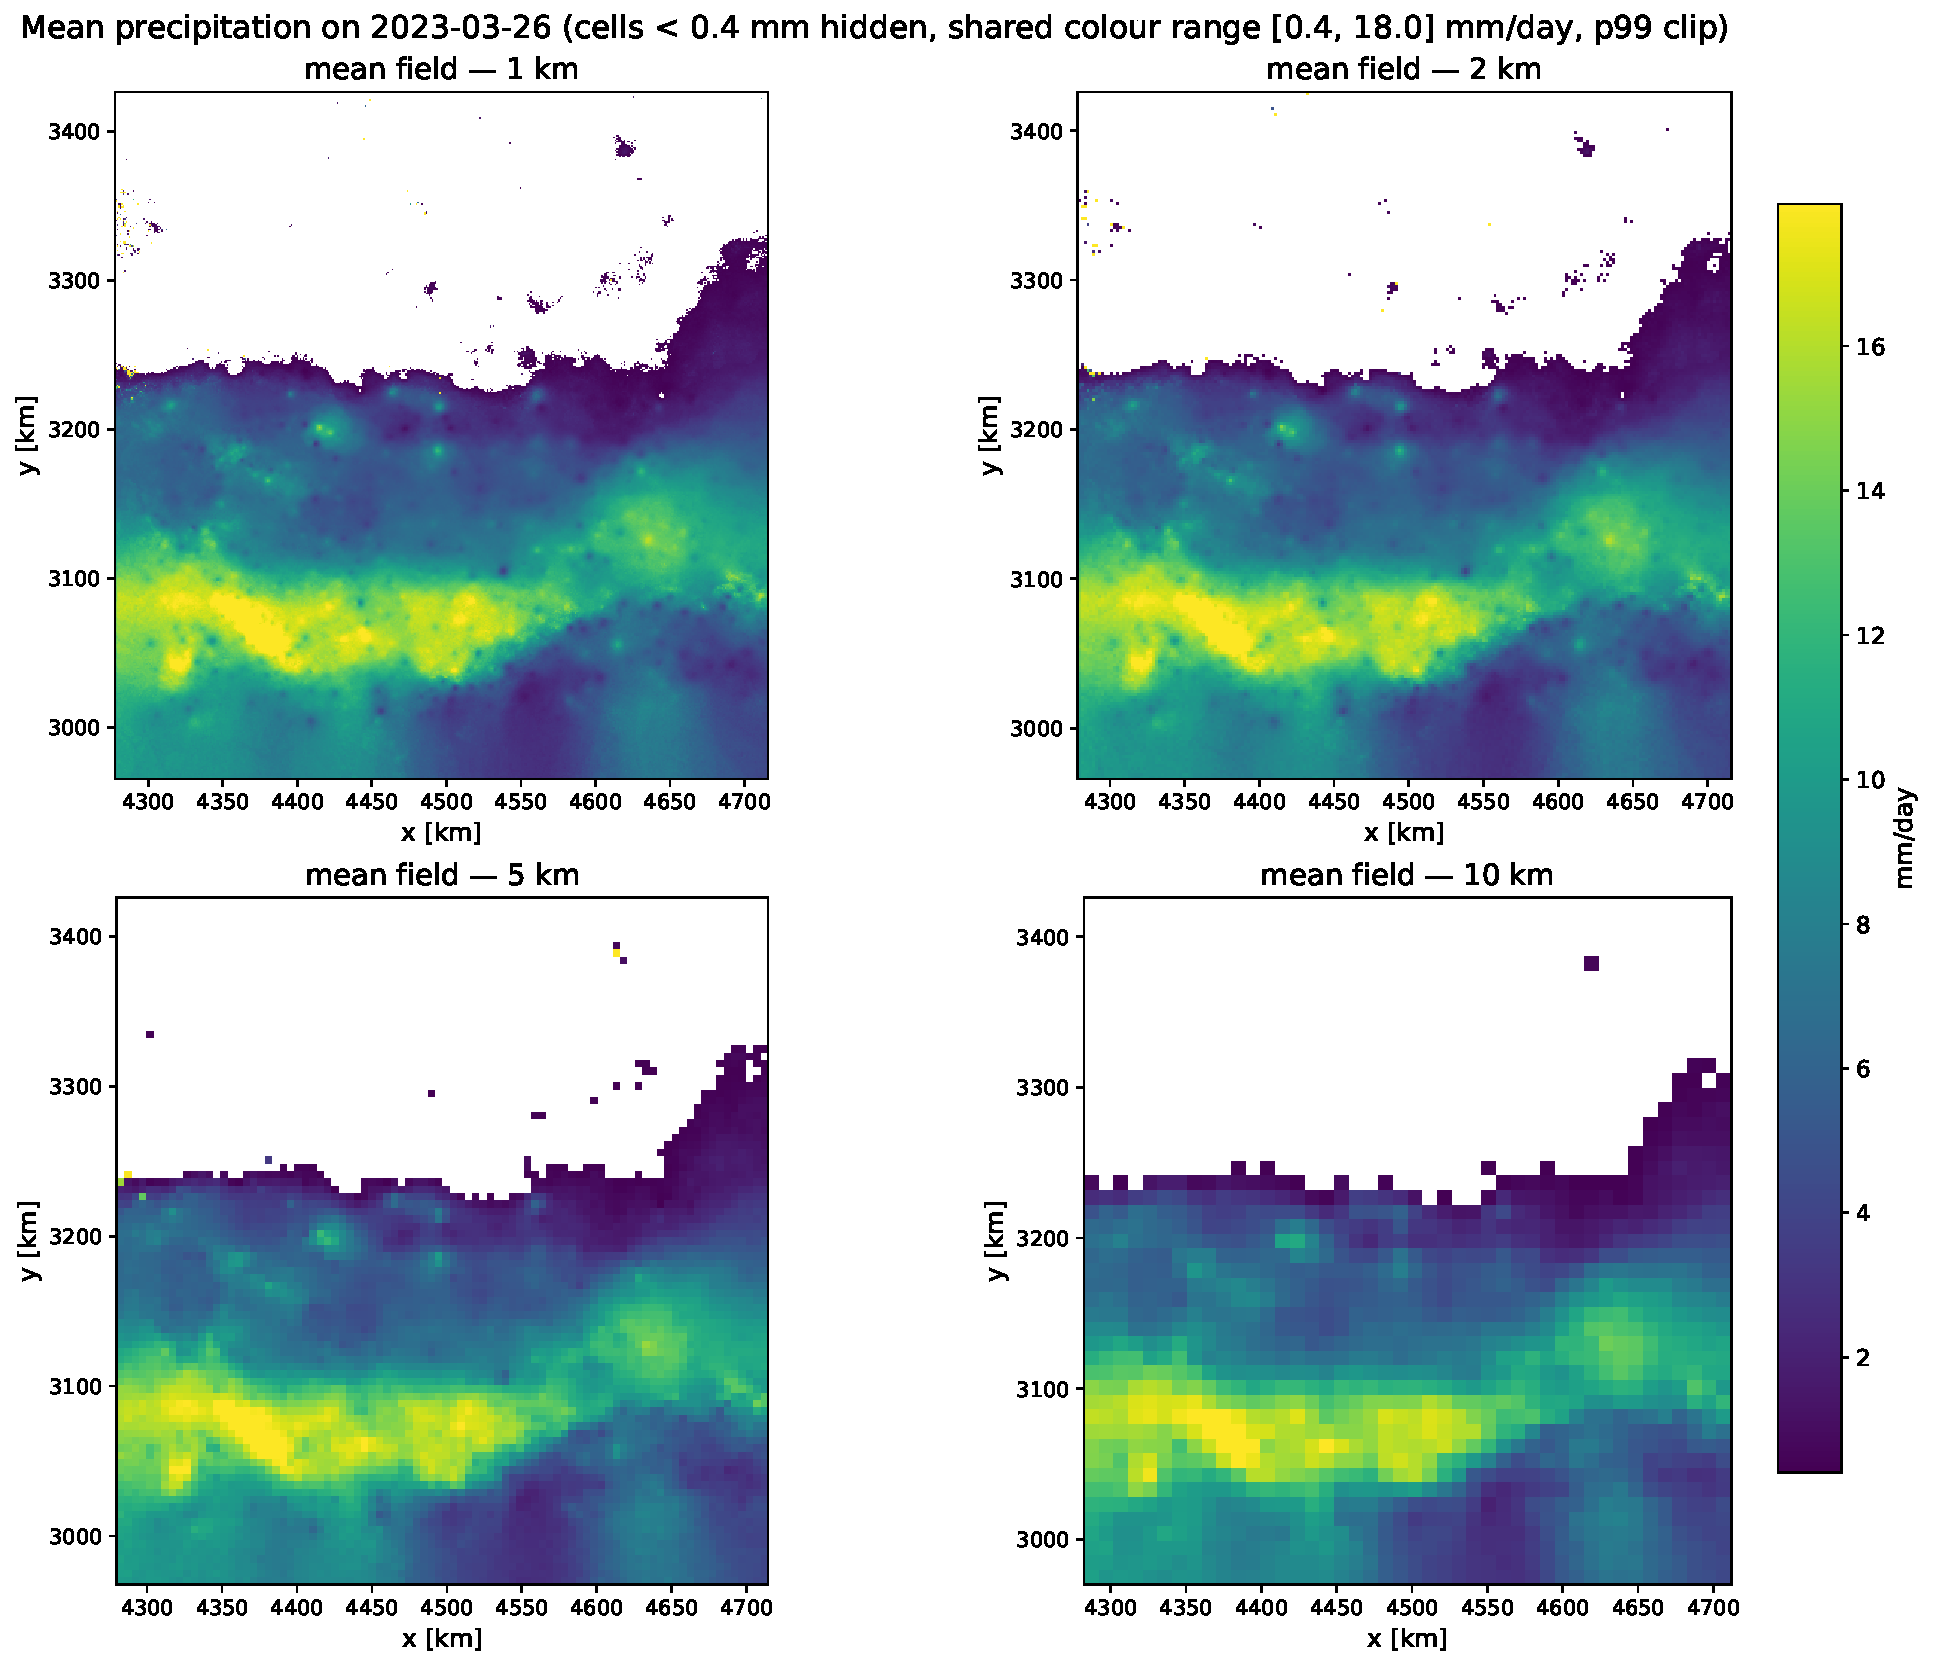
\includegraphics[width=\linewidth]{images/07/multires_case_day.pdf}
  \caption{Posterior mean precipitation on $2023$-$03$-$26$ at the
  four product resolutions ($1$, $2$, $5$ and $10$~km). Cells with
  predicted rainfall below $0.4$~mm are masked. The shared colour
  range $[0.4, 18.0]$~mm clipped at the $99$th percentile lets the
  smoothing of orographic gradients and the gradual loss of small
  isolated rain cells be read off directly between panels.}
  \label{fig:multires-case-day}
\end{figure}

A multi-resolution validation against the holdout stations confirms
that accuracy degrades only modestly with coarsening: holdout MAE
rises from $0.294$~mm at $1$~km to $0.338$~mm at $10$~km, and the bias
between the directly-predicted coarse field and the spatial aggregate
of the $1$~km field stays below $0.02$~mm at every resolution. The
product is distributed as one Parquet file per resolution under
\texttt{results/dataset/predictions\_\{1,2,5,10\}km/}, indexed by
\texttt{(date, cell\_id)}.
